The Web of Things (WoT) architecture~\cite{Wot2017arch} defines three basic entities
that can be organized into various configurations and topologies 
based on a concrete deployment scenario:

\noindent\textbf{$\bullet$ WoT Thing:} Represents a physical or virtual IoT device 
        and exposes a network-facing API for interaction.
	Each WoT Thing has an associated Thing Description (TD)~\cite{Wot2017td}. 
        A TD encodes a set of metadata describing relevant information about a Thing,
        such as semantic categorization, available interactions, and communication and security mechanisms.
        Typically a WoT Thing plays the network role of a server as it responds to
        but does not initiate interactions.
\emph{For example:} 
A WoT Thing might be a garage door controller.
Such a controller would provide a number of interactions that can be performed on a garage door, 
i.e. \textit{open}, \textit{close}, etc. and would provide network interfaces to invoke
each of these.

\noindent\textbf{$\bullet$ WoT Client:} An entity that wants to perform an action on a WoT Thing.
It is able to consume a TD provided by (or for) another WoT Thing and invoke interactions on 
the target's network interfaces.
\emph{For example:} 
A WoT Client might be a browser or an application on a user's smartphone
that allows the user to invoke one of the interactions provided by the above garage door controller. 

\noindent\textbf{$\bullet$ WoT Servient:} Can be viewed as a combination of a client and server:
        an entity that is both providing one or more WoT Thing interfaces (as a server) and
        at the same time is able to operate as WoT Client to invoke interactions on other WoT Things.
\emph{For example:} 
% a WoT Servient might be (a service running on a) home gateway device 
% that acts as a WoT Client towards home appliance WoT Things
% (such as different lights and sensors) and also exposes some higher level ``virtual'' devices 
% in the form of additional WoT Things available for a WoT Client running on a user's smartphone.
A WoT Servient might be a service running on a home gateway device 
that provides a generalized ``lock up'' service (including closing the garage door, but also 
arming the home alarm, securing door locks, turning off lights, etc.) with its own network interface.

Internally a typical architecture of a WoT Servient is shown in Figure~\ref{fig-fservient}. 
In addition to a Thing Description (TD), a full WoT Servient also has WoT Binding Template 
metadata that can be used to instantiate a TD for a particular IoT protocol binding, 
such as OCF, HTTP(S), COAP etc. 

A WoT Servient can also host a WoT Runtime and a WoT Scripting API.
The WoT Scripting API is an optional component that allows 
implementing the logic of an application Servient in a standardized way
using a higher-level programming language (the current WoT draft focuses on JavaScript). 
In this document, however, we focus on the security implications of the metadata alone,
and do not consider further the security implications of the Scripting API (which
raises many issues such as application isolation, prevention of DDoS attacks, and so on).

\begin{figure}[!t]
\centering
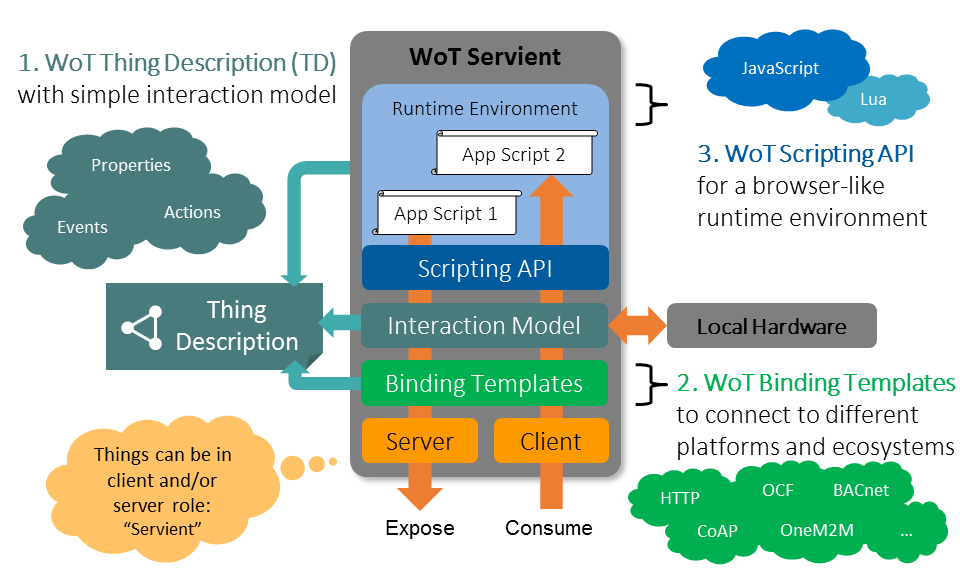
\includegraphics[width=3.3in]{figures/wot-servient.png}
\caption{WoT Servient architecture}
\label{fig-fservient}
\end{figure}


